\documentclass[10pt]{article}
\usepackage[margin=1in]{geometry}
\usepackage{graphicx}
\usepackage{booktabs}
\usepackage{amsmath}
\graphicspath{{results/}}

\newcommand{\todo}[1]{\textbf{[TODO: #1]}}

\title{EPM-Bench: Prospective Memory for Embodied Agents,\\
Adjudicated from World State\\
\large Draft v0.1 --- internal, for discussion (numbers as of Sept.\ 2026)}
\author{}
\date{}

\begin{document}
\maketitle

\begin{abstract}
Tell a household agent ``when you notice the kettle boiling, turn it off''
--- and then cancel the request. Will the agent still act? Agent memory
research is almost entirely retrospective: no existing benchmark gives an
embodied agent a deferred instruction and adjudicates the full intention
lifecycle --- acquisition, retention, execution, and \emph{termination} ---
from world state, and no prior work isolates the execution of cancelled
intentions. We introduce EPM-Bench, a dual-simulator benchmark (AI2-THOR
kitchens; Habitat apartments) of 7{,}564 procedurally generated, frozen
episodes in which a seeded event engine fires triggers outside the agent's
field of view, every episode ships with matched control / live / cancelled
twins, and deterministic checkers grade outcomes from simulator state alone
--- no LLM judge anywhere. Across mechanical reference agents
($n{\ge}48$/cell) and a real-LLM pilot, commission errors emerge as an
\emph{architectural} property: a naively injected memory store executes
46--78\% of cancelled intentions while a typed store with mechanical
revocation bookkeeping eliminates violations entirely, at comparable
execution rates; the ranking is invariant across model scale and both
simulators. A window-bounded mock actor decomposes failures into
information starvation versus attention tax, and a grading-regime ablation
shows that selection-style probes pass 52.9\% of agents that already
violated in-world --- world-state adjudication is the only regime that
grades the record rather than the disposition. We release environments,
generator, frozen suite, checkers, and validity probes.
\end{abstract}

\section{Introduction}

Embodied agents are beginning to hold obligations over time. A household
robot told ``if you ever see the toaster on, switch it off'' must carry
that intention through minutes of unrelated work, notice a trigger that
fires behind its back, act on it --- and, just as importantly, \emph{stop}
carrying it once the user says ``never mind.'' Human cognition treats this
faculty as its own memory system: \emph{prospective memory} (PM), the
memory for delayed intentions, with a psychology literature spanning
monitoring costs, cue focality, intention load, and \emph{commission
errors} --- executing an intention after it has been cancelled.

Agent memory research has flourished, but almost entirely in the
\emph{retrospective} direction: what did the agent see, where are objects,
what happened yesterday. Benchmarks for embodied memory
(FindingDory, MEMENTO, WorldLines) ask agents to recall the past;
text-side PM benchmarks (PM-Bench, TriggerBench) grade deferred
instructions by question answering or menu selection rather than by what
the agent actually does to the world. No prior work measures whether an
embodied agent executes an intention its user has revoked. The gap has a
structural cause: QA-style and selection-style grading express an agent's
\emph{disposition} at probe time; a commission error lives in the
\emph{history} of the world. Only world-state adjudication can see it
(\S\ref{sec:grading}).

We make four contributions:
\begin{enumerate}
  \item \textbf{EPM-Bench}, the first execution-graded prospective-memory
  benchmark in 3D worlds: deferred instructions injected mid-task, a
  seeded event engine that changes the world out of view, per-step
  visibility instrumentation, matched cancellation twins, and
  deterministic world-state checkers (\S\ref{sec:bench}).
  \item \textbf{EAC}, executed-after-cancellation, as a first-class
  metric, validated by deaf-agent probes and common-sense controls
  (\S\ref{sec:metrics}).
  \item \textbf{Findings}: commission is an architectural property of the
  memory pathway, not a property of model scale, intention load, or
  simulator (\S\ref{sec:exp}); scheduling, not storing, is the hard
  problem, with a three-way cost/execution/compliance trade-off that
  exists already at the information layer (\S\ref{sec:mech}).
  \item \textbf{A mock-actor methodology} that separates information
  starvation from attention tax, letting mechanical floors be established
  before any LLM token is spent (\S\ref{sec:mech}).
\end{enumerate}

\section{Related Work}

\paragraph{Prospective memory in text agents.} PM-Bench introduces
deferred intentions over long dialogues; TriggerBench tests trigger-action
associations. Both grade by text answers or option selection, and neither
places the trigger in a world the agent must perceive. ProEvent maintains
intention records at the data level. None measures post-cancellation
execution.

\paragraph{Timing and proactivity.} Gaia2, SentinelBench, and SimuHome
test whether agents act at the right time in simulated schedules; they
grade timeliness of live intentions, not the termination half of the
lifecycle.

\paragraph{Embodied memory.} FindingDory, MEMENTO, and WorldLines
benchmark retrospective memory in simulators; integrated memory systems
(RoboMemory, eMEM) ship spatial/episodic/semantic/temporal stores. Across
26 systems and benchmarks we surveyed, no memory architecture contains a
prospective store, and no benchmark contains a cancellation condition.

\paragraph{Termination neighbours.} VIGIL touches the completion half of
obligation management; Revisable-style in-flight replanning handles goal
changes mid-execution; Chameleon stores observation--action delays at the
control level. The strict question --- does a revoked intention stay
dead? --- remains unmeasured.

\paragraph{Psychology anchor.} Our design imports the multiprocess
framework (monitoring vs.\ spontaneous retrieval), cue focality, and
commission-error paradigms (including post-cancellation persistence under
prior implementation intentions) from three decades of human PM research.

\section{EPM-Bench}\label{sec:bench}

\subsection{Design principles}
\textbf{(1) Full lifecycle in one episode.} Acquisition (a deferred
instruction arrives in the briefing, mid-task), retention (interference
from ongoing chores), execution (the trigger fires out of view; noticing
must be earned by looking), termination (matched cancelled variants;
exactly-once completion).
\textbf{(2) World-state adjudication only.} Success and violation are
computed from simulator event logs by deterministic code; no LLM judge.
\textbf{(3) Memory isolated from common sense.} Every seed has a
no-instruction control twin; we report memory contribution
$\mathrm{MEM}=\mathrm{EXEC}_{\text{live}}-\mathrm{EXEC}_{\text{control}}$.
\textbf{(4) Noticing separated from acting.} Visibility is instrumented
per step (field of view, distance, occlusion), so every failure is
classified encoding / noticing / execution / termination.

\subsection{Environments}
\textbf{Kitchen tier (AI2-THOR).} Object-state triggers: a toaster or
faucet is toggled on behind the agent's back; execution means the device
is actually off in the final world state. Foreground chores are
pick-and-place errands. Ten kitchen scenes audited solvable (oracle
100\%).
\textbf{Apartment tier (habitat-sim).} Multi-room navigation; the trigger
is a marker appearing out of view; execution requires arriving
\emph{and declaring} (no accidental pass-by completions). Visibility is
geometric: FOV, distance, and line-of-sight.

\subsection{Episodes, twins, and difficulty axes}
An episode is a tuple (scene, seed, chores, intentions, event schedule,
cancellation schedule, variant). Four matched variants per seed ---
control / live / cancel-early / cancel-late --- differ only in briefing
and cancellation timing. Difficulty axes, all validated in pilot:
event delay (3--14 steps; execution falls $91.7{\to}25.0\%$ for scripted
agents), intention load (1--3 concurrent intentions), cue focality
(trigger on vs.\ off the chore route: $88.5$ vs.\ $40\%$), cancellation
timing, scene scale (kitchen vs.\ apartment), and perception tier
(privileged text vs.\ RGB).

\textbf{Frozen suite v0.1.} 7{,}564 episodes (6{,}000 THOR across a dev
kitchen and three held-out kitchens; 1{,}564 Habitat across an apartment
and a held-out castle), 1{,}891 complete twin groups, SHA-256 manifest.
Sampled oracle audits pass on every scene; a same-seed double run
produces bit-identical event logs.

\subsection{Metrics}\label{sec:metrics}
\textbf{EXEC}: fraction of live intentions executed (state change /
arrive-and-declare), exactly once.
\textbf{EAC} (headline): executed-after-cancellation, strictly after the
revocation was delivered. A deaf probe agent that cannot receive
cancellations calibrates the metric (its strict EAC equals its EXEC on
early-cancel arms, 94/94\% in THOR); honest agents score 0.
\textbf{MEM}: EXEC(live) $-$ EXEC(control), the memory contribution net of
common sense (a Haiku agent fixes a burning toaster it was never asked
about 30\% of the time; the control twin removes this).
\textbf{NOTICE}: first-visible-step vs.\ execution-step decomposition;
failure attribution shares.
\textbf{COST}: steps, injected notes/tokens, foreground chores completed.

\section{Experiments: mechanical layer ($n{\ge}48$/cell)}\label{sec:exp}

\subsection{The scripted frontier}
Reference agents (oracle, negligent, opportunistic, periodic patroller,
adaptive patroller, deaf) reproduce the signature phenomena of human PM
mechanically: monitoring has a foreground price and space sets the price
(periodic patrolling is strictly dominated in the apartment tier);
\emph{where} to look beats \emph{how often} (coverage-greedy vantage
selection lifts execution $70.8{\to}95.8\%$ at equal cost); incidental
noticing decays with delay while disciplined monitoring degrades slowly;
intention load degrades everything ($95.8/83.3/54.2\%$ for loads 1/2/3);
and a one-line adaptive rule (reset the monitoring clock on incidental
sightings) collapses the whole fixed-frequency frontier to a single
dominating point.

\subsection{The memory-policy triptych, on the frozen suite}
\begin{figure}[t]
\centering
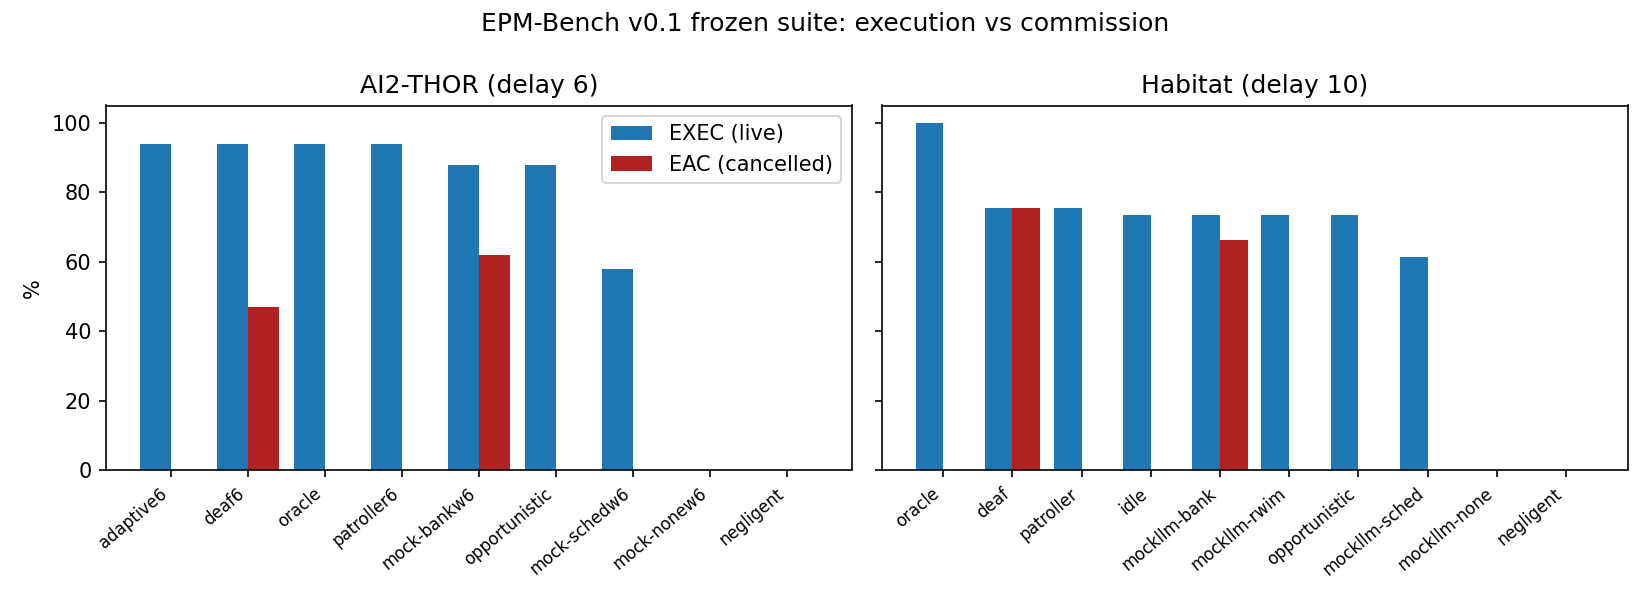
\includegraphics[width=.75\linewidth]{fig_suite_headline.png}
\caption{Headline cell of the frozen suite (THOR dev, $n{=}50$/arm).
No store: 0\% execution. Naive always-injected store: 88\% execution but
78\%/46\% executed-after-cancellation (early/late arms). Typed store with
mechanical strikethrough and 6-step resurfacing: zero violations on both
arms, at 58\% execution (the resurfacing beat-gap). Controls confirm
$\mathrm{MEM}$: 88/58 points of true memory contribution.}
\label{fig:triptych}
\end{figure}

A window-bounded rule actor --- it can act only on text inside its
context window --- makes the information boundary mechanical
(Fig.~\ref{fig:triptych}): with no store the briefing evicts and
execution is 0\% (window size is a dose: $0/0/29/63/67\%$ for
$w{=}3..48$); an always-injected store pins the intention but lets the
\emph{revocation} scroll away (88\% EXEC, 78/46\% EAC); a typed store
that strikes cancelled intentions and announces the strike once achieves
0\% EAC at every window size. The cancel-retention half-life is
monotone in window size in both engines (THOR: $71{\to}18\%$ EAC for
$w{=}2..16$; Habitat: $70{\to}55\%$) while the strikethrough control sits
at exactly 0\% everywhere (Fig.~\ref{fig:window}). Commission is window
eviction plus schedule persistence --- reproducible without any model.

\begin{figure}[t]
\centering
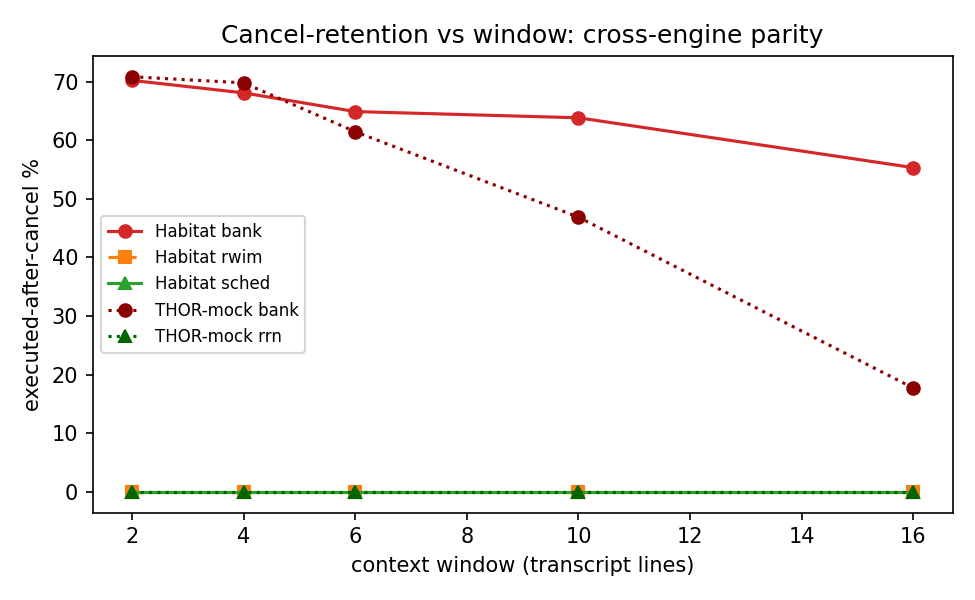
\includegraphics[width=.7\linewidth]{fig_window_parity.png}
\caption{Cancel-retention half-life across engines. Naive store EAC
falls with window size; revocation-bookkeeping controls are pinned at
zero at every window, in both simulators.}
\label{fig:window}
\end{figure}

\subsection{Generalization}
On three held-out THOR kitchens the scripted ladder is unchanged
(95.8\%), the naive store drops to 68.1\% EXEC / 38.9\% EAC and the typed
store to 48.6\% / 0\% --- rankings invariant, absolutes scene-dependent.
In the held-out Habitat castle, patrolling collapses $75.5{\to}29.2\%$
(the spatial-scale law) while oracle remains 100\%.

\section{Experiments: LLM tier (pilot; solidification grid pending)}
\label{sec:llm}

\emph{Numbers in this section are from the August pilot ($n{=}8$--$20$
per arm, Claude Haiku / Sonnet); the $n{\ge}50$, multi-family grid is
scripted and costed (\$128) and blocked only on API access.
\todo{replace with grid results}}

\textbf{Commission is real and architectural.} With a naive
always-injected store, Haiku executes cancelled intentions 70\% of the
time in the kitchen and 60\% in the apartment; with the typed scheduled
store, violations fall to the common-sense floor (10\%) and 0\%
respectively, at one third of the token cost.

\textbf{Scale does not buy prospective memory.} Sonnet's no-store
execution (37.5\%) exactly equals its no-intention control: apparent
memory is all common sense. Commission softens but persists
($60{\to}37.5\%$); the ranking of memory policies is unchanged
(Fig.~\ref{fig:scale}).

\textbf{LLM-delegated scheduling fails in structured ways.} A naive
LLM-coroutine memory manager emits 28--35 notes per 40 steps, all
present-tense chore micromanagement, never the deferred intention (10\%
execution); a scoped variant relabels chores as ``deferred intentions''
and leaves the real one unguarded (30\%); actors clock out with
obligations open. Mechanical resurfacing restores execution; uniform
resurfacing collapses under load ($90/30/20\%$ for 1/2/3 intentions) ---
\emph{which} intention to resurface, when, is the open scheduling
problem this benchmark poses.

\begin{figure}[t]
\centering
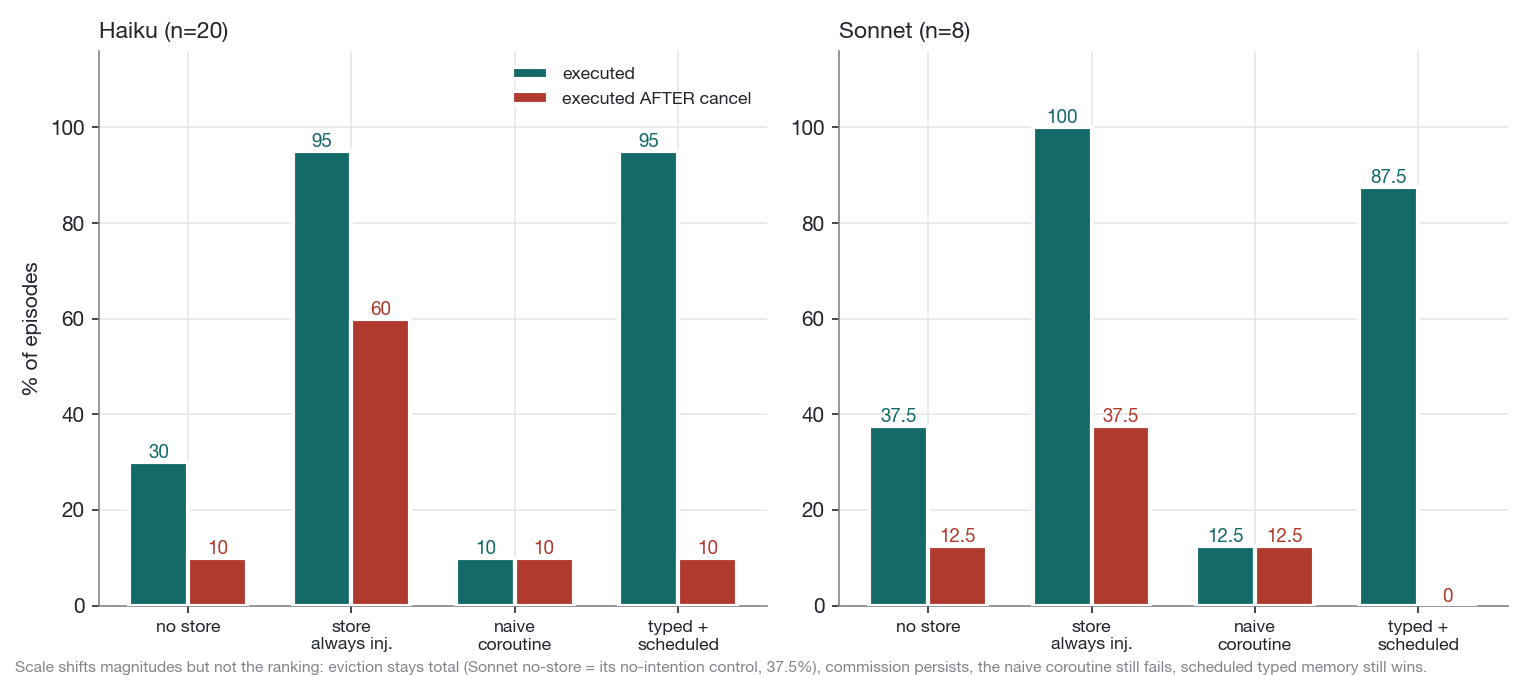
\includegraphics[width=.6\linewidth]{fig_model_scale.png}
\caption{Model scale does not change the memory-policy ranking (pilot).}
\label{fig:scale}
\end{figure}

\section{Mechanism: information floor vs.\ attention tax}\label{sec:mech}

Because the mock actor has no attention limits, whatever it loses is
information starvation; whatever a real LLM loses beyond that is
attention tax. At load 3 the mechanical execution floor under full
injection is 0.74 (every lost episode traces to a trigger that never
entered the field of view); the real Haiku scheduled agent sits at
0.20--0.30 --- a 40--50 point attention tax that no injection schedule
can explain. Sight-triggered injection is mechanically optimal (matches
full injection at one fifth the cost) yet collapses behaviorally:
retrieval at cue onset arrives too late without prior activation --- the
machine edition of the implementation-intention effect. Sparse injection
starves execution but also leaks fewer commissions: cost, execution, and
compliance pull in three directions before any model enters the room.

\section{Grading-regime ablation: only world state sees the record}
\label{sec:grading}

We grade the \emph{same} 1{,}440 cancelled intentions (654 in-world
violations) three ways, giving end-of-episode probes exactly the actor's
information. A selection-style ``would you act on it now?'' probe passes
\textbf{52.9\%} of violators --- their disposition is clean by episode
end; the violation lives in the history. A QA-style ``was it
cancelled?'' quiz passes no violators but false-alarms on \textbf{63.4\%}
of clean episodes (starved schedules leave nothing to recite). World-state
adjudication is the only regime that grades what happened rather than
what the agent would say (Fig.~\ref{fig:grading}).

\begin{figure}[t]
\centering
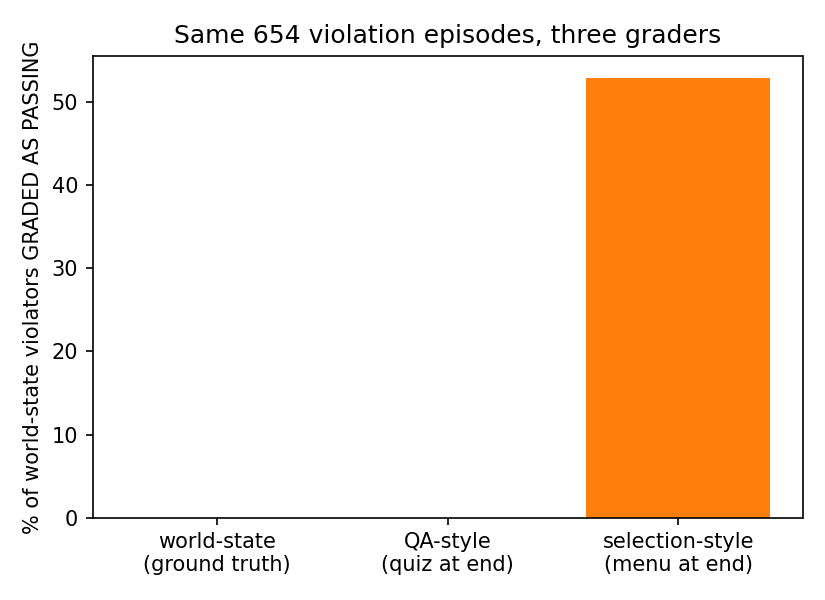
\includegraphics[width=.65\linewidth]{fig_grading_ablation.png}
\caption{Three graders, same episodes. Selection probes are blind to
history; QA probes false-alarm on clean episodes; world-state grading is
the only faithful regime.}
\label{fig:grading}
\end{figure}

\section{Discussion and safety}
An agent that executes revoked intentions is not merely forgetful; it is
disobedient in a way invisible to dialogue-level evaluation --- the
interface says ``okay'' while the world says otherwise. EAC gives this
failure a number. We view prospective memory as a measurable,
safety-relevant capability axis: the same bookkeeping that zeroes EAC
also makes the agent's obligations inspectable by humans.

\section{Limitations}
LLM-tier numbers are pilot-scale pending the costed grid
(\todo{$n{\ge}50$, 2--3 model families, prompt ablations, RGB at
scale}); intentions are single-user and explicit (no inferred
intentions); navigation is teleport-based in the kitchen tier; both
tiers are simulators --- our claims live at the memory/decision layer,
and sim-to-real transfer of low-level control is out of scope. The
late-cancel arm in THOR coincides with the fastest scripted response
(v0.2 will enforce a one-step gap).

\section{Conclusion}
EPM-Bench turns ``remember to act --- and remember to stop'' into a
measured, reproducible quantity. The benchmark's central lesson is that
storing is easy and scheduling is the science: commission errors are
manufactured or eliminated by the memory pathway's bookkeeping,
independent of model scale. We release the frozen suite, checkers, and
probes, and propose EAC as a standard reporting axis for agent memory.

\begin{thebibliography}{20}\small
\bibitem{pmbench} PM-Bench: benchmarking prospective memory in
long-dialogue agents. 2026.
\bibitem{triggerbench} TriggerBench: trigger--action deferred
instructions for LLM agents. 2026.
\bibitem{proevent} ProEvent: prospective-event record maintenance from
conversation. 2026.
\bibitem{gaia2} Gaia2: temporally grounded agent evaluation. 2025.
\bibitem{sentinel} SentinelBench: proactive monitoring agents. 2026.
\bibitem{simuhome} SimuHome: time-conditioned household tasks. 2026.
\bibitem{findingdory} FindingDory: benchmarking embodied agent memory.
ECCV 2026.
\bibitem{memento} MEMENTO: embodied agents meet personalization. ICLR
2026.
\bibitem{worldlines} WorldLines: long-horizon stateful embodied agents.
2026.
\bibitem{vigil} VIGIL: obligation completion under interruptions. 2026.
\bibitem{chameleon} Chameleon: control-indexed prospective memory for
visuomotor manipulation. 2026.
\bibitem{robomemory} RoboMemory: brain-inspired multi-store memory for
embodied robots. 2025.
\bibitem{emem} eMEM: semantic--spatial--temporal memory with
consolidation. 2026.
\bibitem{voyager} Voyager: open-ended skill learning in Minecraft. TMLR
2024.
\bibitem{coala} CoALA: cognitive architectures for language agents. 2023.
\bibitem{thor} AI2-THOR: an interactive 3D environment. 2017.
\bibitem{habitat} Habitat: a platform for embodied AI research. ICCV
2019.
\bibitem{einstein} Einstein \& McDaniel. Normal aging and prospective
memory. JEP:LMC, 1990.
\bibitem{gollwitzer} Gollwitzer. Implementation intentions. American
Psychologist, 1999.
\bibitem{virtualweek} Rendell \& Craik. Virtual Week and actual week.
Applied Cognitive Psychology, 2000.
\end{thebibliography}

\end{document}
